\ignore{From real-case observations, we discover several relational
constraints among concept relations that can be used to enforce the
relation between two input concepts identified by our relation
classifier.}

\ignore{Analyzing concepts and the relations between them reveals
  several relational constraints among the relations identified for
  the target pair and those identified for related concepts. }

The key insight of the inference model is that if we have more than
two concepts, only some kinds of relations between them are
possible. For instance, {\em George W. Bush} cannot be an ancestor or
sibling of {\em president} if we are confident that {\em president} is
an ancestor of {\em Bill Clinton}, and {\em Bill Clinton} is a sibling
of {\em George W. Bush}. We call the combination of concepts and their
relations a {\em concept network}. Figure \ref{fig:triangles} shows some
$n$-node concept networks consisting of two input concepts ($x$, $y$),
and additional concepts $z$, $w$, $v$. \ignore{In general, $n$
  concepts can be involved to construct $n$-node concept networks ($n
  > 2$). In this paper, we focus on $3$-node concept networks
  consisting of the two target concepts and an additional
  one. However, our formalization applies to general $n$-node concept
  networks.}

\ignore{From our observations, we see that if we can obtain additional
  concepts in addition to the two input concepts, we can enforce such
  relational constraints as prior knowledge to guide the final
  decision of the relation identifier. In the literature, several
  models take advantage of prior knowledge to achieve significant
  improvement in performance
  \cite{DenisBa07,CGRT09}. There are two main
  approaches to inject prior knowledge. The first approach
  incorporates prior knowledge {\em indirectly}; by adding more
  features \cite{RothYi05}. The other incorporates prior knowledge
  {\em directly} in the form of hard or soft constraints
  \cite{ChangRaRo08}. We want to incorporate prior knowledge directly,
  therefore our model is closely related to the latter approach.}

The aforementioned observations show that, if we can obtain additional
concepts that are related to the two input concepts, we can enforce
such relational constraints as prior knowledge to make a global
prediction on the taxonomic relation of two given concepts. Our
inference model follows constraint-based formulations that were
introduced in the NLP community and were shown to be very effective in
exploiting declarative background knowledge
\cite{RothYi04,DenisBa07,PunyakanokRoYi08,ChangRaRo08}.

\ignore{While it is also possible to inject prior knowledge {\em
    indirectly}, by adding more features, it has been argued (e.g.,
  \cite{RothYi05,ChangRaRo08}) that a {\em direct} way, in the form of
  soft or hard constraints, is beneficial due to better expressiveness
  and simpler learning. Our model follows this approach.}

\begin{figure}[!t]
  \centering
  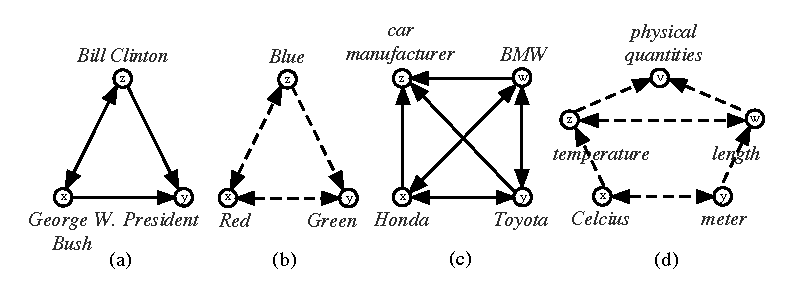
\includegraphics[totalheight=0.107\textheight]{networks}
  \caption{Examples of $n$-node concept networks with two
      input concept $x$ and $y$. Networks (a) and (c) show valid
      combinations of edges, whereas (b) and (d) are two relational
      constraints. For simplicity, we do not draw {\em no relation}
      edges in (d).}
  \label{fig:triangles}
\end{figure}

\subsection{Constraints as Prior Knowledge}
\label{sec:cons-prior-know}
Let $x, y$ be two input concepts, and $\mathcal{Z}=\{z_1, z_2, ...,
z_m\}$ be a set of additional concepts. For a subset $Z \in
\mathcal{Z}$, we construct a set of concept networks whose nodes are
$x$, $y$ and all elements in $Z$, and the edge, $e$, between every two
nodes is one of four taxonomic relations whose weight, $w(e)$, is
given by a local classifier (Sec. \ref{sec:learning}). If $l = |Z|$,
there are $n=2+l$ nodes in each network, and $4^{\left [ \frac{1}{2}
    n(n-1) \right ] }$ concept networks can be constructed. We only
focus on 3-node concept networks (i.e. $l = 1$). For example, for
input pair ({\em red}, {\em green}) and $\mathcal{Z} = \{ blue, yellow
\}$, we can construct 64 networks for triple $\left < red, green,
  Z=\{blue\} \right >$ and 64 networks for $\left < red, green,
  Z=\{yellow\} \right >$ by trying all possible relations between the
concepts.

\ignore{For a subset $Z \in \mathcal{Z}$, a set of concept networks is
  constructed. Each concept network contains two input concepts $x$,
  and $y$, and all additional concepts in $Z$. Every two concepts in a
  concept network are connected by their relations which are the four
  relations of interest in this paper. A local relation classifier is
  used to give weights for 4 relation classes of an edge in a concept
  network. We use $e$ and $w(e)$ to denote an edge in a concept
  network and its corresponding weight, respectively. If $n$ is the
  number of concepts in a network ($n > 2$), there will be $4^{\left [
      \frac{1}{2} n(n-1) \right ] }$ concept networks that can be
  constructed because there are $4$ relations for every $2$ concepts.
  With $m=1$, each network consists of 3 nodes, and there are $64$
  concept networks.}
%

A {\em relational constraint} is defined as a concept network, by
regarding only its edges' setting, that belongs to a pre-defined list
of invalid edges' combinations. For example, Figure
\ref{fig:triangles}b shows an invalid network where {\em red} is a
sibling of both {\em green} and {\em blue}, and {\em green} is an
ancestor of {\em blue}. In Figure \ref{fig:triangles}d, {\em Celcius}
and {\em meter} cannot be siblings because they are children of two
sibling concepts {\em temperature} and {\em length}. The relational
constraints used in our experiments are manually constructed.

\ignore{Figure \ref{fig:triangles}(b) demonstrates a relational
  constraint where the combination of edges is ({\em sibling}, {\em
    sibling}, {\em ancestor}) moving clockwise direction with respect
  to $x$ and $y$.}

Let $\mathcal{C}$ be a list of relational constraints. Equation (\ref{eqn:tscore}) defines the network scoring function,
which is a linear combination of the edge weights, $w(e)$, and the
penalties, $\rho_k$, of concept networks matching constraint $C_k \in
\mathcal{C}$.

\begin{equation}
  \label{eqn:tscore}
  score(t) = \sum_{e \in t} w(e) - \sum_{k=1}^{|\mathcal{C}|} \rho_{k} d_{C_k}(t)
\end{equation}

function $d_{C_k}(t)$ indicates if $t$ matches $C_k$. In our work, we
use relational constraints as hard constraints and set their penalty
$\rho_k$ to $\infty$. For a set of concept networks formed by $\left <
  x, y, Z \right >$ and all possible relations between the concepts,
we select the best network, $t^* = \text{argmax}_tscore(t)$.

\ignore{Eqn. \ref{eqn:tscore} allows us to pick the best
setting of all edges connecting concepts in the networks with respect
to $\mathcal{C}$.}

After picking the best concept network $t^*$ for every $Z \in
\mathcal{Z}$, we make the final decision on the taxonomic relation
between $x$ and $y$. Let $r$ denote the relation between $x$ and $y$
in a particular $t^*$ (e.g. $r = x \leftrightarrow y$.) The set of all
$t^*$ is divided into 4 groups with respect to $r$ (e.g. a group of
all $t^*$ having $r=x \leftrightarrow y$, a group of all $t^*$
having $r=x \leftarrow y$.) We denote a group with concept networks
holding $r$ as the relation between $x$ and $y$ by
$\mathcal{T}_{r}$. To choose the best taxonomic relation, $r^*$, of
$x$ and $y$, we solve the objective function defined in Equation
\ref{eqn:objectivefunction}.

\ignore{ After collecting all the topmost concept networks by going
  through all $Z \in \mathcal{Z}$, the topmost concept networks are
  divided into four groups with respect to the relation of $x$ and $y$
  in each network. Each group of the topmost concept networks is
  denoted by $\mathcal{T}_{r}$. To make the final decision
  concerning the relation of two input concepts $(x,y$), we solve the
  objective function defined in Eqn. \ref{eqn:objectivefunction}.}

\begin{equation}
  \label{eqn:objectivefunction}
  r^* = \text{argmax}_{r} \frac {1} {|\mathcal{T}_{r}|} \sum_{t^* \in \mathcal{T}_{r}} \lambda_{t^*} score(t^*)
\end{equation}

\ignore{
{\small
\begin{eqnarray}
\label{eqn:objectivefunction}
r^* & = & \text{argmax}_{r} \frac {1} {|\mathcal{T}_{r}|} \sum_{t \in \mathcal{T}_{r}} \lambda_{t} score(t) \\
& = & \text{argmax}_{r} \frac{1}{|\mathcal{T}_{r}|} \sum_{t \in \mathcal{T}_{r}} \lambda_{t} \left( \sum_{e \in t} w(e) - \sum_{k=1}^{|\mathcal{C}|} \rho_{k} d_{C_k}(t) \right) \notag
\end{eqnarray}
}
}

where $\lambda_t$ is the weight of concept network $t$, defined as the
occurrence probability of $t$ (regarding only its edges' setting) in
the training data, which is augmented with additional
concepts. Equation (\ref{eqn:objectivefunction}) finds the best
taxonomic relation of two input concepts by computing the average
score of every group of the best concept networks representing a
particular relation of two input concepts. \ignore{In general,
  $n$-node concept networks can be selected as relational constraints
  and used in our inference model. But one can always decompose
  $n$-node networks into $3$-node networks to allow greedy search in
  the concept network space.}

\ignore{

  To measure $\lambda_t$, a local relation classifier is used to
  predict the best relation between concepts in the concept networks
  in the training data.

  \begin{equation}
    \lambda_t = \frac{\# \text{ of occurrences of }t}{\# \text{ of
        predicted concept networks in training data}} \notag
  \end{equation}
}

\ignore{
\subsection{Constraint Selection}
\label{sec:constraintselection}

In Eqn. (\ref{eqn:objectivefunction}), a list of relational
constraints $\mathcal{C}$ is used. Recall that a relational constraint
is an invalid concept network that is not allowed to happen. In our
work, relational constraints are mined from the training data by
applying the {\em forward feature selection} technique discussed in
\cite{944968}. The algorithm starts with an empty set of constraints
$\mathcal{C}$, then grows the constraint set gradually by including in
the set the {\em best} concept network from each iteration. The {\em
  best} concept network is defined as the constraint used in
Eqn. (\ref{eqn:objectivefunction}) that improves the system's
performance most. Our {\em forward constraint selection} algorithm is
described in Figure \ref{alg:forwardselection}. Function
\texttt{evaluate}($\mathcal{D}$, $\mathcal{L}$, $\mathcal{C}$)
evaluates the system on all examples and their related concepts in
$\mathcal{D}$ using a trained local classifier $\mathcal{L}$ with
respect to a set of constraints $\mathcal{C}$ by solving the objective
function in Eqn. (\ref{eqn:objectivefunction})

\begin{figure}[!t]
  \begin{centering}
    {\scriptsize
      \fbox{
        \begin{minipage}{6in}
          \begin{tabbing}
            {Algorithm \textsc{Forward Constraint Selection}} \\
            \qquad {\textsc{Input}}: Data set with related concepts $\mathcal{D} = \left < (x, y, r, \mathcal{Z}) \right >$ ~~~~~\\
            \qquad \qquad A trained local relation classifier $\mathcal{L}$. \\
            \qquad \qquad A list of concept networks $\mathcal{T} = \{ t_1, t_2, \dots, t_{m} \}$; \\
            \qquad {\textsc{Output}}: Constraint set $\mathcal{C}$. \\
            \\
            \qquad $\mathcal{C} = \emptyset$; {\em isIncreasing} = true; \\
            \qquad {\em bestAcc} = \texttt{evaluate}($\mathcal{D}$, $\mathcal{L}$, $\mathcal{C}$); \\
            \qquad While ({\em isIncreasing}) do \\
            \qquad \qquad {\em isIncreasing} = false; \\
            \qquad \qquad For each $t \in \mathcal{T}$ do \\
            \qquad \qquad \qquad $\mathcal{C} = \mathcal{C} \cup \{ t \}$; \\
            \qquad \qquad \qquad {\em acc} = \texttt{evaluates}($\mathcal{D}$, $\mathcal{L}$, $\mathcal{C}$); \\
            \qquad \qquad \qquad If ({\em acc} $>$ {\em bestAcc}) then \\
            \qquad \qquad \qquad \qquad $t^* = t$; {\em isIncreasing} = true; \\
            \qquad \qquad \qquad \qquad {\em bestAcc} $=$ {\em acc}; \\
            \qquad \qquad \qquad End if \\
            \qquad \qquad \qquad $\mathcal{C} = \mathcal{C} \backslash \{ t \}$; \\
            \qquad \qquad End for \\
            \qquad \qquad If ({\em isIncreasing}) then \\
            \qquad \qquad \qquad $\mathcal{C} = \mathcal{C} \cup \{ t^* \}$; $\mathcal{T} = \mathcal{T} \backslash \{ t^* \}$; \\
            \qquad \qquad End if \\
            \qquad End while \\
            \\
            \qquad \textsc{Return}: $\mathcal{C}$; \\
          \end{tabbing}
        \end{minipage}
      }
    }
  \end{centering}
  \caption{
    \label{alg:forwardselection}
    Forward constraint selection algorithm. Function
    \texttt{evaluate}($\mathcal{D}$, $\mathcal{L}$, $\mathcal{C}$)
    evaluates the system on all examples and their related concepts in
    $\mathcal{D}$ using a trained local classifier $\mathcal{L}$ with
    respect to a set of constraints $\mathcal{C}$ by solving
    Eqn. (\ref{eqn:objectivefunction}).}
\end{figure}

One of the inputs of the algorithm, $\mathcal{T}$, is a set of $m$
concept networks. At each iteration, all concept networks $t \in
\mathcal{T}$ are tried; at the end of the iteration, the {\em
  best} network is added to $\mathcal{C}$ and removed from
$\mathcal{T}$. In this paper, for simplicity, we only use 3-node
concept networks, thus, $m = 64$. In general, $n$-node concept
networks can also be selected as relational constraints and used in
our model by decomposing $n$-node networks into $3$-node
networks to allow greedy search performed in the concept network
space.
}

\subsection{Extracting Related Concepts}
\label{sec:rel-con-ext}

To apply our constraint-based inference model, we need to acquire
concepts additional to the input pair. From now on, we refer to
additional concepts as {\em related concepts}. The related concept
space is defined as a space of direct ancestors, siblings and children
in a particular resource.

\ignore{In principle, with strong relational constraints and a
  reasonable local taxonomic relation classifier, one can use random
  concepts as additional concepts to do inference. However, there is a
  high chance that a random additional concepts will simply produce
  {\em no relation} with two input concepts, and eventually will not
  help the inference model.  \ignore{To address this issue, we
    investigate different approaches to obtain additional concepts
    which are related to input concepts.}  Our experiment (see
  Sec. \ref{sec:experiments} shows that the proposed inference model
  gets better results when doing inference with additional concepts
  that are more relevant to input concepts.}


\ignore{ In the first direction, as the first step to verifying the
  correctness of our proposed constraint-based inference model, we
  manually add {\em gold related concepts}, which are very related to
  input concepts. By using {\em gold related concepts}, a significant
  improvement in the system's performance is necessary to prove the
  correctness of the inference model. Our experiments (see
  Sec. \ref{sec:contr-relat-conc}) following this direction indeed
  prove that our proposed inference model is correct and accurate.  }

\begin{figure}[!t]
  \begin{centering}
    {\scriptsize
      \fbox{
        \begin{minipage}{6in}
          \begin{tabbing}
            \textsc{Yago} \textsc{Query Patterns} \\
            \qquad \textsc{Input:} concept ``$X$'' \\
            \qquad \textsc{Output:} lists of ancestors, siblings, and children of ``$X$'' ~~~~~~~~~~~~~~~~~~ \\
            \\
            \qquad \begin{tabular}{l|l|l}
              Pattern 1 & Pattern 2 & Pattern 3 \\
              \hline
              ``$X$'' \textsc{means} \texttt{?A} & ``$X$'' \textsc{means} \texttt{?A} & ``$X$'' \textsc{means} \texttt{?D} \\
              \texttt{?A} \textsc{subclassof} \texttt{?B} &  \texttt{?A} \textsc{type} \texttt{?B} & \texttt{?E} \textsc{type} \texttt{?D}  \\
              \texttt{?C} \textsc{subclassof} \texttt{?B} & \texttt{?C} \textsc{type} \texttt{?B} & \\
            \end{tabular}
            \\
            \\
            \qquad \textsc{Return:} \texttt{?B}, \texttt{?C}, \texttt{?E} as \\
            \qquad \qquad \qquad lists of ancestors, siblings, and children, respectively. \\
          \end{tabbing}
        \end{minipage}
      }
    }
  \end{centering}
  \caption{Our \textsc{Yago} query patterns used to obtain related concepts for ``$X$''.}
  \label{alg:yago-query}
\end{figure}

\ignore{However, in real world applications, {\em gold related
    concepts} are not available.}

We propose an approach that uses the \textsc{Yago} ontology
\cite{suchanek2007WWW} to provide related concepts. It is worth noting
that \textsc{Yago} is chosen over the Wikipedia category system used
in our work because \textsc{Yago} is a clean ontology built by
carefully combining Wikipedia and lexical database
WordNet.\footnote{However, \textsc{Yago} by itself is weaker than our
  approach in identifying taxonomic relations (see
  Sec. \ref{sec:experiments}.)}

In \textsc{Yago} model, all objects (e.g. {\em cities}, {\em people},
etc.)  are represented as {\em entities}. To map our input concepts to
entities in \textsc{Yago}, we use \textsc{means} relation defined in
\textsc{Yago} ontoloy. Furthermore, similar entities are grouped into
{\em classes}. This allows us to obtain direct ancestors of an entity
by using \textsc{type} relation which gives the entity's
classes. Furthermore, we can get ancestors of a class with
\textsc{subclassof} relation\footnote{These relations are defined in
  the \textsc{Yago} ontology.}. By using three relations
\textsc{means}, \textsc{type} and \textsc{subclassof} in \textsc{Yago}
model, we can obtain direct ancestors, siblings, and children, if any,
of an input concept. Figure \ref{alg:yago-query} presents three
patterns that we used to query related concepts from \textsc{Yago}
ontology. \ignore{For concepts having no children, such as {\em honda
    civic}, {\em bill clinton}, we simple ignore their children.}

% By default, we use this approach to provide related concepts for our
% constraint-based inference model.

\ignore{
\begin{figure}[!t]
  \begin{centering}
    {\scriptsize
      \fbox{
        \begin{minipage}{6in}
          \begin{tabbing}
            \textsc{Yago} \textsc{Query Patterns} \\
            \qquad \textsc{Input:} concept ``$X$'' \\
            \qquad \textsc{Output:} lists of ancestors, siblings, and children of ``$X$'' ~~~~~~~~~~~~~~~~~~ \\
            \\
            \qquad \textsc{Pattern 1:} \\
            \qquad \qquad ``$X$'' \textsc{means} \texttt{?A} \\
            \qquad \qquad \texttt{?A} \textsc{type} \texttt{?B} \\
            \qquad \qquad \texttt{?C} \textsc{type} \texttt{?B} \\
            \qquad \textsc{Pattern 2:} \\
            \qquad \qquad ``$X$'' \textsc{means} \texttt{?D} \\
            \qquad \qquad \texttt{?E} \textsc{type} \texttt{?D} \\
            \\
            \qquad \textsc{Return:} \texttt{?B}, \texttt{?C}, \texttt{?E} as \\
            \qquad \qquad \qquad lists of ancestors, siblings, and children, resp. \\
          \end{tabbing}
        \end{minipage}
      }
    }
  \end{centering}
  \caption{Our \textsc{Yago} query patterns used to obtain lists of direct ancestors,
    siblings, and children for concept $X$.}
  \label{alg:yago-query}
\end{figure}
}

\ignore{
In Figure \ref{alg:yago-query}, \textsc{Pattern 1} is used to get lists
of ancestors and siblings of a given concept.  For example, with
concept ``$X$''= ``{\em honda civic}'', \textsc{Pattern 1} returns
lists of ancestors \linebreak[4] \{{\em wikicat\_1970s\_automobiles,
  wn\_car\_102958343, \linebreak[4] wikicat\_Honda\_vehicles,
  $\dots$}\}, and siblings \linebreak[4] \{{\em Ford\_Capri,
  Mercury\_Comet, Honda\_Jazz, Honda\_Accord, $\dots$}\}. The prefix
and suffix annotation of the ancestors are dropped.  In the case that
ancestors are noun phrases, we only use the head of the phrase. We use
the Noun Group parser from \cite{suchanek2007WWW} to extract the {\em
  head} of a noun phrase. In the other hand, \textsc{Pattern 2}
returns an empty list of children of ``{\em honda civic}'', because
its corresponding entity \texttt{Honda\_Civic} is at the deepest level
in \textsc{Yago} ontology. The list of children will be non-empty if
``$X$'' is some generic concept such as ``{\em actor}'', ``{\em
  president}'', etc.
}

%%% Local Variables:
%%% mode: latex
%%% TeX-master: "jupiter"
%%% End:
